\documentclass[11pt,a4paper]{article}
\usepackage[utf8]{inputenc}
\usepackage[T1]{fontenc}
\usepackage{lmodern}
\usepackage{amsmath,amssymb}
\usepackage{booktabs}
\usepackage{array}
\usepackage{enumitem}
\usepackage{geometry}
\usepackage{graphicx}
\usepackage{hyperref}
\usepackage{microtype}
\usepackage{xcolor}
\usepackage{tikz}
\usetikzlibrary{arrows.meta,positioning,fit,backgrounds,shapes.geometric,calc}
\geometry{margin=1in}
\hypersetup{colorlinks=true,linkcolor=blue,citecolor=blue,urlcolor=blue}

\title{Decoupling Learning from Inference:\\\Large The Rise of On-Device Meta-Learning Paradigms for Agents}
\author{PaperX Working Draft}
\date{April 2026}

\begin{document}

\maketitle

\begin{abstract}
Most deployed AI agents still behave like systems with powerful but largely static weights. They can reason over context, retrieve documents, and call tools, yet they rarely adapt their internal computation in real time to the particular user, environment, or sensor stream in front of them. This creates a growing mismatch between deployment conditions and learning mechanisms: real-world agents increasingly live on phones, wearables, robots, and embedded systems, while the dominant machinery of learning remains full backpropagation over large parameter spaces in datacenter settings.

This paper argues for a different architectural split. Heavy representation learning, meta-training, and robustness tuning should remain offline or in the cloud, while fast adaptation should happen locally during inference through memory writes, latent-state updates, and hyper-network-conditioned modulation. In this view, the relevant unit of online adaptation is not the entire parameter tensor of the model, but a smaller adaptive substrate that can steer a frozen backbone. Hyper-networks, fast weights, external memory, adapters, and test-time adaptation methods all point toward this broader shift from weight-centric learning to state-centric plasticity.

We synthesize prior work in meta-learning, test-time training, hyper-networks, parameter-efficient adaptation, memory-augmented models, and recent self-updating LLMs, and we connect these lines to current on-device AI deployment stacks from Apple, Google, and Qualcomm. The central claim is that the next generation of hardware-constrained agents will become adaptive not by running conventional full training loops on device, but by decoupling heavy learning from real-time inference and moving lightweight meta-learning mechanisms into local state. This shift improves personalization, latency, energy efficiency, and privacy, and it suggests a path from static digital assistants toward agents with bounded but meaningful cognitive plasticity. A public copy of this paper is available at \url{https://github.com/xiaol/Autoresearch_ideas/blob/main/papers/on_device_meta_learning_agents/paper58.pdf}.
\end{abstract}

\section{Introduction}

Large foundation models are trained as if intelligence is mainly a property of weights. The expensive part of learning happens before deployment; afterward, the model is expected to generalize. This approach has delivered extraordinary performance, but it breaks down in an important regime: agents that must adapt continuously after deployment.

The problem is especially visible for edge agents. A phone assistant, wearable coach, home device, or mobile robot does not inhabit the average conditions of a benchmark. It inhabits one user's routines, one room layout, one speech profile, one sensor stack, one schedule, and one evolving set of local constraints. A frozen model may be broadly capable, yet still feel strangely rigid because it cannot efficiently internalize these narrow but consequential regularities.

This paper argues that the bottleneck is not merely scale; it is architectural coupling. Today, ``learning'' is too often equated with the machinery of full training, while ``inference'' is treated as a read-only execution phase. We propose a different framing: heavy learning and real-time adaptation should be decoupled. Base competence can remain in frozen pretrained weights, but deployment-time adaptation should be delegated to lighter mechanisms that modify state, memory, routing, or low-dimensional control variables.

\begin{figure}[t]
\centering
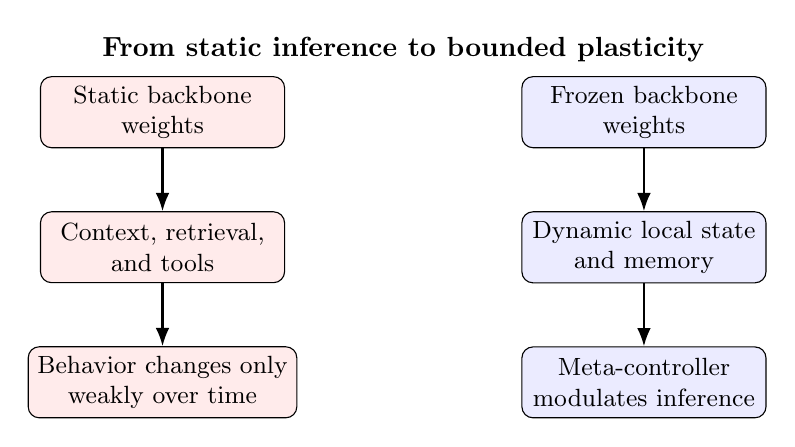
\begin{tikzpicture}[
    font=\small,
    box/.style={draw, rounded corners, align=center, minimum width=3.1cm, minimum height=0.9cm},
    arr/.style={-Latex, thick}
]
\node[box, fill=red!8] (left1) {Static backbone\\weights};
\node[box, fill=red!8, below=0.8cm of left1] (left2) {Context, retrieval,\\and tools};
\node[box, fill=red!8, below=0.8cm of left2] (left3) {Behavior changes only\\weakly over time};

\node[box, fill=blue!8, right=3.0cm of left1] (right1) {Frozen backbone\\weights};
\node[box, fill=blue!8, below=0.8cm of right1] (right2) {Dynamic local state\\and memory};
\node[box, fill=blue!8, below=0.8cm of right2] (right3) {Meta-controller\\modulates inference};

\draw[arr] (left1) -- (left2);
\draw[arr] (left2) -- (left3);
\draw[arr] (right1) -- (right2);
\draw[arr] (right2) -- (right3);

\node[align=center, font=\bfseries] at ($(left1)!0.5!(right1)+(0,0.8)$) {From static inference to bounded plasticity};
\end{tikzpicture}
\caption{Two deployment regimes. The left stack reflects the common pattern in which a frozen model uses more context but does not substantially alter its internal behavior. The right stack shows the paper's target regime: a frozen backbone steered by writable local state and a meta-controller.}
\label{fig:static_vs_plastic}
\end{figure}

This is not a claim that online learning is new. Meta-learning, test-time training, fast weights, external memory, and parameter-efficient tuning all provide precedents. Nor is it a claim that every useful adaptation can or should be purely local. Instead, the contribution of this paper is a synthesis and a systems-level thesis:

\begin{quote}
The most practical route to adaptive on-device agents is to move from direct online weight training toward online state modulation, with heavy optimization remaining offline and lightweight plasticity happening at inference time.
\end{quote}

We present this as a position paper rather than an experimental system report. Our goal is to bridge several research lines that are often discussed separately and show why, taken together, they motivate a new paradigm for hardware-constrained agents.

\section{The Problem-Solution Gap}

\subsection{Why Current Agents Feel Static}

Modern agents often appear adaptive because they can retrieve history, expand context windows, or chain tools. But these mechanisms are not the same as changing the computation that produces behavior. Retrieval reintroduces information; it does not necessarily alter the model's internal control policy. Prompting reshapes the immediate context; it does not reliably internalize recurring local structure. Tool use extends capability; it does not by itself grant plasticity.

This is why users often encounter a familiar contradiction: a model can solve advanced tasks, yet fail to absorb a simple preference or repeated environmental regularity over time. Inference remains powerful, but the boundary between seeing new evidence and changing behavior is still too brittle.

\subsection{The Energy Asymmetry of Learning}

The standard recipe for neural learning remains expensive. Gradient-based adaptation requires forward and backward passes, optimizer state, and parameter updates over large tensors. On edge hardware, this creates an energy asymmetry: bounded inference can be optimized for low latency and controlled thermal behavior, while conventional online training is persistent, memory-hungry, and power-intensive.

This mismatch matters because edge devices operate under battery, heat, and responsiveness constraints. Apple frames Core ML around on-device execution that minimizes memory footprint and power consumption, while also supporting stateful models and efficient execution of transformer operations on device \cite{apple_coreml}. Google AI Edge similarly emphasizes reducing latency, working offline, and keeping data local and private across mobile, web, and embedded deployments \cite{google_edge}. Qualcomm's recent device materials explicitly tie a faster Hexagon NPU and on-device AI learning features to more personalized and power-efficient ``agentic AI'' experiences \cite{qualcomm_2025}. These platform directions reinforce a simple point: the edge stack is being optimized for efficient local adaptation, not for transplanting the full datacenter training loop into a phone.

\subsection{The Weights-versus-States Dilemma}

The result is a false binary:
\begin{itemize}[noitemsep]
    \item keep the model frozen and efficient, but weakly personalized; or
    \item retrain the model, but only rarely and at high infrastructure cost.
\end{itemize}

This binary is too coarse for agent deployment. Many important forms of personalization are local, reversible, user-specific, and time-sensitive. A device may need to learn speech habits, explanation preferences, notification priorities, household routines, daily biometric baselines, gesture conventions, or common task sequences. These do not always belong in globally shared weights. They are often better modeled as state.

Ba et al. make a closely related distinction in their fast-weights work, contrasting standard slow weights with faster-changing forms of memory that can store recent information without rewriting the whole model \cite{ba2016fastweights}. We use the term \emph{weights-versus-states dilemma} to generalize that intuition to modern agents: if useful adaptation must always be written into weights, adaptation will remain too slow and expensive for the edge; if adaptation can instead be written into state, then plasticity becomes much more feasible.

\section{Related Work}

\subsection{Meta-Learning and Fast Adaptation}

Meta-learning established the principle that systems can be trained to adapt quickly rather than merely to perform well in a single frozen configuration. MAML made this explicit by learning parameters that are easy to adapt with a small number of gradient steps on a new task \cite{finn2017maml}. Later work addressed the computational burden of inner-loop differentiation, including implicit-gradient formulations \cite{rajeswaran2019implicit}. Although classical meta-learning is rarely framed as an edge systems strategy, its core lesson is directly relevant here: some of the burden of future adaptation can be moved into offline training.

This paper extends that lesson in a systems direction. Instead of asking how to make full online gradient adaptation efficient enough for the edge, we ask how offline meta-learning can prepare a model to adapt primarily through local state changes.

\subsection{Hyper-Networks and Dynamic Conditioning}

Hyper-networks provide a natural mechanism for this shift because they turn one network into a generator or modulator of another network's parameters or activations. Ha et al. formalized hyper-networks as models that generate weights for a main network \cite{ha2016hypernetworks}. Dynamic Filter Networks similarly generate input-conditioned filters rather than keeping all filters fixed after training \cite{jia2016dynamic}. FiLM showed that feature-wise affine modulation can exert strong control over downstream reasoning without replacing the entire backbone \cite{perez2018film}. More recent work such as HyperTransformer applies model generation directly in few-shot settings \cite{zhmoginov2022hypertransformer}.

These methods differ in scope, but they share the same architectural insight: behavior can be changed by generating or modulating a smaller control surface rather than by retraining the full base model. That is precisely the kind of mechanism that becomes attractive on constrained hardware.

\subsection{Test-Time Training and Test-Time Adaptation}

Test-time adaptation takes a different route to the same goal: letting a trained model adapt after deployment when the test distribution shifts. Test-Time Training introduced self-supervised adaptation at test time to improve generalization under distribution shift \cite{sun2020ttt}. Tent pushed this further by optimizing prediction entropy at test time, updating a restricted subset of parameters online \cite{wang2021tent}. MT3 explicitly combined meta-learning, self-supervision, and test-time training in a single framework \cite{bartler2022mt3}.

These methods are important precedents because they reject the strict train-then-freeze boundary. However, most of them still assume some form of online optimization. The perspective advanced here is more deployment-oriented: test-time adaptation is useful, but edge agents will often need even lighter mechanisms than repeated gradient updates on live devices.

\subsection{Parameter-Efficient Tuning}

Parameter-efficient tuning methods offer another bridge between static pretraining and local adaptation. Adapters showed that small task-specific modules can achieve competitive transfer without fine-tuning all parameters \cite{houlsby2019adapters}. LoRA further reduced trainable state by learning low-rank updates with strong empirical efficiency \cite{hu2021lora}. Meta-Adapters imported meta-learning into this parameter-efficient setting by learning adapter modules that can adapt effectively in few-shot regimes while keeping the backbone frozen \cite{bansal2022metaadapters}.

These methods are usually discussed as fine-tuning strategies, not as real-time agent substrates. Still, they demonstrate an important systems principle: large behavior changes can often be induced by updating a tiny fraction of the model. Our claim is that edge agents should push this logic further, toward deployment-time adapter state, routing state, and latent modulation that can be updated locally with bounded cost.

\subsection{External Memory, Fast Weights, and Self-Updating Models}

Another major line of work replaces direct parameter editing with richer memory mechanisms. Neural Turing Machines and Differentiable Neural Computers coupled neural controllers to writable external memory \cite{graves2014ntm, graves2016dnc}. One-shot Memory-Augmented Neural Networks showed that rapid assimilation can be achieved through memory rather than repeated relearning of the full model \cite{santoro2016mann}. Fast weights introduced a third memory timescale between activations and slow weights, explicitly framing temporary associative memory as a distinct substrate \cite{ba2016fastweights}. Metalearned Neural Memory went further by treating memory itself as a rapidly adaptable function updated in one shot \cite{munkhdalai2019mnm}. Long-context architectures such as Transformer-XL and Compressive Transformer extended the memory horizon of sequence models by caching or compressing prior states \cite{dai2019transformerxl, rae2019compressive}.

Recent LLM work has begun to reconnect these ideas to deployment-time adaptation. MEMORYLLM argues that LLMs ``usually remain static after deployment'' and introduces a transformer with a fixed-size latent memory pool designed to self-update with injected knowledge \cite{wang2024memoryllm}. MAC is especially close to our thesis: it adapts a frozen language model during test time by storing compact modulations in a memory bank, using amortization-based meta-learning to replace what would otherwise require optimization with a single forward pass \cite{tack2024mac}. In our view, MAC is one of the clearest concrete demonstrations that the field is moving from direct retraining toward modulation-based online adaptation.

\subsection{In-Context Learning as Inference-Time Adaptation}

In-context learning already demonstrates that substantial adaptation-like behavior can emerge at inference time even when weights stay fixed. Li et al. formalize this lens by analyzing transformers as algorithms operating on contextual examples \cite{li2023icl}. We do not equate in-context learning with persistent local adaptation, but it reinforces the larger argument of this paper: useful behavioral change can be induced through state and context without immediately touching the base parameterization.

\subsection{Edge AI Platforms}

Finally, platform trends matter. Apple's tooling now explicitly supports stateful models, efficient execution of transformer operations, and on-device execution that minimizes memory and power consumption \cite{apple_coreml}. Apple also publicly discussed on-device personalization years earlier, including fine-tuning on device for user-specific concepts \cite{apple_wwdc19}. Google AI Edge presents on-device deployment as a way to reduce latency, work offline, and keep data local and private, while exposing hardware-accelerated pipelines and support for on-device generative models \cite{google_edge}. Qualcomm's recent platform materials explicitly link NPU gains and sensing-hub learning features to more personalized on-device agentic AI \cite{qualcomm_2025}. These are not proofs of our thesis, but they are strong market signals that the deployment stack is aligning with it.

\section{Decoupling Learning from Inference}

The practical implication of the literature above is not that online gradient descent disappears. It is that the system can be re-partitioned.

\paragraph{Offline phase.}
The cloud or training cluster should continue to carry the heavy burden: representation learning, meta-training, robustness tuning, compression, distillation, and optimization of adaptation policies.

\paragraph{Online phase.}
The device should perform lighter operations: updating short- and medium-term memory, maintaining latent summaries, selecting or generating modulation codes, adjusting adapters or routing coefficients, and composing local state with a frozen backbone.

This creates a three-layer picture of deployed intelligence:
\begin{enumerate}[noitemsep]
    \item \textbf{Base weights} for broad competence and long-horizon priors.
    \item \textbf{Dynamic state} for recent experience, local environment, and user-specific regularities.
    \item \textbf{Meta-controller} for deciding how state should steer ongoing inference.
\end{enumerate}

The crucial move is to treat the third layer as the main substrate of deployment-time learning. A hyper-network, modulation encoder, or memory controller can be trained offline so that, at deployment time, it converts local evidence into small but high-leverage changes in computation.

\begin{figure}[t]
\centering
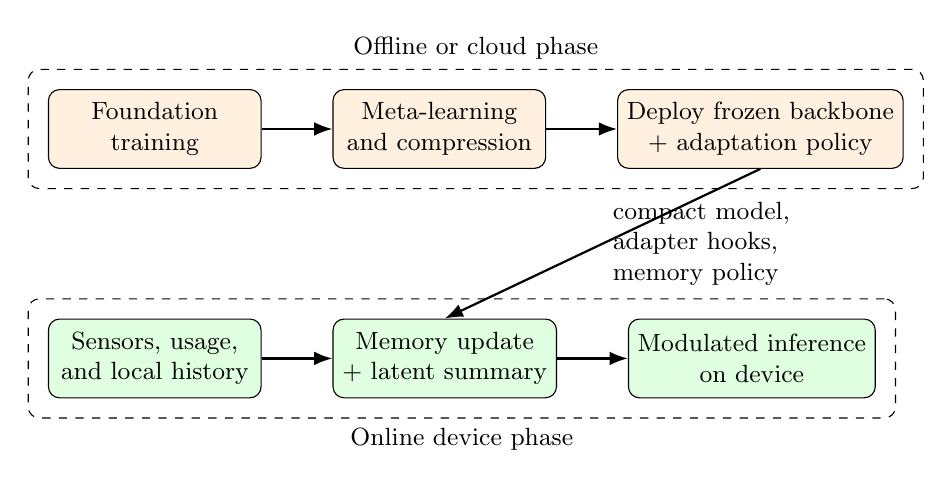
\begin{tikzpicture}[
    font=\small,
    stage/.style={draw, rounded corners, align=center, minimum width=2.7cm, minimum height=1.0cm},
    arr/.style={-Latex, thick}
]
\node[stage, fill=orange!12] (cloud1) {Foundation\\training};
\node[stage, fill=orange!12, right=0.9cm of cloud1] (cloud2) {Meta-learning\\and compression};
\node[stage, fill=orange!12, right=0.9cm of cloud2] (cloud3) {Deploy frozen backbone\\+ adaptation policy};

\node[draw, dashed, rounded corners, fit=(cloud1)(cloud2)(cloud3), inner sep=0.25cm, label=above:{Offline or cloud phase}] {};

\node[stage, fill=green!12, below=1.9cm of cloud1] (dev1) {Sensors, usage,\\and local history};
\node[stage, fill=green!12, right=0.9cm of dev1] (dev2) {Memory update\\+ latent summary};
\node[stage, fill=green!12, right=0.9cm of dev2] (dev3) {Modulated inference\\on device};

\node[draw, dashed, rounded corners, fit=(dev1)(dev2)(dev3), inner sep=0.25cm, label=below:{Online device phase}] {};

\draw[arr] (cloud1) -- (cloud2);
\draw[arr] (cloud2) -- (cloud3);
\draw[arr] (dev1) -- (dev2);
\draw[arr] (dev2) -- (dev3);
\draw[arr] (cloud3.south) -- node[right, align=left] {compact model,\\adapter hooks,\\memory policy} (dev2.north);
\end{tikzpicture}
\caption{Decoupling learning from inference. Heavy optimization remains offline, while the device updates memory and latent control state at run time.}
\label{fig:decoupling_pipeline}
\end{figure}

\begin{table}[t]
\centering
\small
\begin{tabular}{>{\raggedright\arraybackslash}p{2.4cm} >{\raggedright\arraybackslash}p{3.1cm} >{\raggedright\arraybackslash}p{2.8cm}}
\toprule
\textbf{Adaptation regime} & \textbf{What changes online} & \textbf{Edge fit} \\
\midrule
Full retraining & Large parameter tensors and optimizer state & Poor \\
PEFT fine-tuning & Small adapters or low-rank weights & Moderate \\
Test-time training & Restricted parameters through online optimization & Moderate \\
State modulation & Memory, latent codes, routing, gates, or activations & Strong \\
\bottomrule
\end{tabular}
\caption{Why state-centric adaptation is attractive on constrained devices.}
\label{tab:regimes}
\end{table}

Table~\ref{tab:regimes} summarizes the central systems argument. Full retraining is the wrong primitive for most devices. State-centric modulation is not necessarily weaker; in many deployment settings it is the only regime that matches the latency, energy, and privacy constraints of the substrate.

\section{The Architecture of Plasticity}

\subsection{Hyper-Networks as ``Brain Above the Brain''}

A useful way to think about on-device meta-learning is as a two-level control architecture. The backbone stores general competence. Above it sits a smaller network that interprets local evidence and decides how the backbone should behave now. This upper layer need not regenerate the whole model. It can output per-layer gains, adapter coefficients, attention biases, routing choices, memory write strengths, or low-dimensional latent keys.

\begin{figure}[t]
\centering
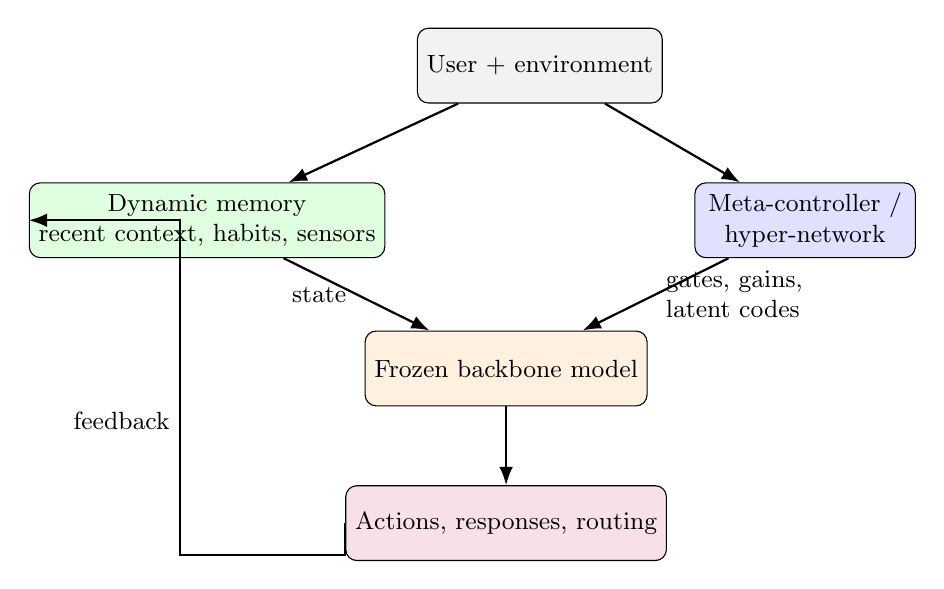
\begin{tikzpicture}[
    font=\small,
    box/.style={draw, rounded corners, align=center, minimum width=2.8cm, minimum height=0.95cm},
    arr/.style={-Latex, thick}
]
\node[box, fill=gray!10] (user) {User + environment};
\node[box, fill=green!12, below left=1.0cm and 0.4cm of user] (memory) {Dynamic memory\\recent context, habits, sensors};
\node[box, fill=blue!12, below right=1.0cm and 0.4cm of user] (meta) {Meta-controller /\\hyper-network};
\node[box, fill=orange!12, below=1.4cm of $(memory)!0.5!(meta)$] (backbone) {Frozen backbone model};
\node[box, fill=purple!12, below=1.0cm of backbone] (action) {Actions, responses, routing};

\draw[arr] (user) -- (memory);
\draw[arr] (user) -- (meta);
\draw[arr] (memory) -- node[left] {state} (backbone);
\draw[arr] (meta) -- node[right, align=left] {gates, gains,\\latent codes} (backbone);
\draw[arr] (backbone) -- (action);
\draw[arr] (action.west) |- ++(-2.1,-0.4) |- node[pos=0.2,left] {feedback} (memory.west);
\end{tikzpicture}
\caption{Internal architecture of local plasticity. The backbone remains mostly fixed, while dynamic memory and a smaller meta-controller reshape behavior through state and modulation.}
\label{fig:plasticity_arch}
\end{figure}

Such a system does not change what the model knows in the long run every time a new event occurs. Instead, it changes how the model uses what it knows. This is why hyper-network-style adaptation is attractive: it relocates the burden of plasticity from massive global tensors to a smaller set of high-leverage control variables.

\subsection{Memory Update Instead of Weight Update}

The key computational substitution is simple:
\begin{itemize}[noitemsep]
    \item traditional online learning writes into weights;
    \item on-device meta-learning writes into memory and control state.
\end{itemize}

This is not just an engineering compromise. It is often the correct abstraction. Many deployment-time regularities are ephemeral or highly local. A wearable adjusting to today's physiological baseline, a phone assistant learning a user's current travel routine, or a home robot disambiguating a new object arrangement often benefits more from rapid reversible memory writes than from permanent changes to the global model.

\subsection{Latent State Modulation}

Latent-state modulation provides a practical implementation path. The device maintains a compact state summarizing recent interactions, uncertainty, user preferences, and environmental cues. That state is then injected into the backbone through one or more mechanisms:
\begin{itemize}[noitemsep]
    \item feature-wise affine modulation,
    \item low-rank activation transforms,
    \item recurrent hidden-state editing,
    \item writable key-value memory,
    \item expert routing over sub-policies,
    \item retrieval-conditioned latent summaries.
\end{itemize}

From the user's perspective, this can look like continuous learning. Strictly speaking, the base model may still be frozen. Functionally, however, the system becomes plastic because its inference trajectory is persistently shaped by accumulated local state.

\section{Hardware-Constrained Evolution}

The timing of this shift is not accidental. Edge AI stacks are increasingly designed around low-power inference, model compression, heterogeneous acceleration, and stateful execution rather than around unrestricted training loops.

Apple's current Core ML materials explicitly highlight stateful models, support for adapters, efficient execution of transformer operations, and dispatch to CPU, GPU, and Neural Engine in ways that minimize memory and power consumption \cite{apple_coreml}. Google's AI Edge stack emphasizes on-device deployment, local privacy, hardware accelerators, and accelerated pipelines that can run across mobile, web, and embedded environments \cite{google_edge}. Qualcomm's 2025 product brief connects an upgraded Hexagon NPU and sensing-hub learning features to personalized agentic experiences, alongside stated gains in performance-per-watt \cite{qualcomm_2025}.

These sources are platform documents rather than controlled scientific comparisons, so we cite them as evidence of deployment direction rather than proof of any one architectural thesis. The larger inference is straightforward: the hardware and software ecosystem is increasingly prepared to support bounded local adaptation, especially when that adaptation is expressed as memory access, modulation, and small auxiliary computation.

This matters because the edge power envelope is unforgiving. For interactive agents, staying in the single-digit watt range is often far more realistic than sustaining repeated backward passes over large models. The design question should therefore be reframed. We should not ask how to miniaturize conventional training until it fits every device. We should ask how to redesign adaptation so that the online phase is natively compatible with the hardware.

\section{The Sovereignty of Local Logic}

\subsection{Privacy}

Local adaptation changes the privacy story because the adaptation trace need not leave the device. Sensitive signals such as speech patterns, location habits, household routines, keystroke rhythms, or physiological baselines are often precisely the information that should not be centralized merely to make the agent more useful.

When adaptation happens through device-local state instead of cloud retraining, privacy becomes an architectural property rather than only a legal or policy overlay. This is one reason official platform messaging consistently links on-device execution with privacy preservation \cite{apple_coreml, google_edge, apple_wwdc19}.

\subsection{Personalized Intelligence}

The most valuable signals for personalization are often too noisy, too private, or too individualized to justify incorporation into global foundation weights. That is exactly why they belong in local logic. A genuinely personalized agent should be able to pivot its reasoning based on evidence that exists only on one device for one person.

\subsection{Security and Self-Repair}

Local plasticity also suggests a new security posture. If an agent can adjust constrained control pathways or memory policies on device, then some local failure modes may be mitigated without waiting for a new global model release. This should not be confused with unconstrained self-modification; the relevant design goal is bounded self-repair with rollback, auditing, and conservative write policies. The broader lesson is that plasticity can support reliability if it is treated as a controlled systems interface rather than as unrestricted autonomy.

\section{Toward Cognitive Plasticity}

The long-term implication of this shift is that deployed agents become less like static instances of one model and more like locally diverging descendants of a shared prior. Every device begins from similar base competence but follows its own adaptation history through memory, modulation, and local control updates.

This does not require romantic claims about consciousness or open-ended self-evolution. A more modest statement is enough: once an agent persistently reshapes how it interprets, plans, and responds based on accumulated local state, it crosses an important threshold from static assistance toward bounded cognitive plasticity.

In that regime, the user's experience changes in three ways:
\begin{enumerate}[noitemsep]
    \item the agent becomes faster because many adaptations happen without a server round trip;
    \item the agent becomes more personal because sensitive local signals can inform behavior directly;
    \item the agent becomes more continuous because experience can accumulate in structured state instead of vanishing at the end of a session.
\end{enumerate}

The paper's stronger forward-looking claim is therefore not that each device will train a wholly new model. It is that a shared foundation can branch into many locally differentiated agents whose identities are carried by state as much as by weights.

\section{Research Agenda}

Several open problems determine whether this paradigm becomes robust engineering practice.

\paragraph{Stable versus plastic substrates.}
Future systems need principled decompositions between what should remain frozen, what should be slowly updateable, and what should be rapidly rewritten.

\paragraph{Evaluation.}
Static benchmarks are poorly matched to adaptive agents. We need evaluations for adaptation speed, power cost, privacy preservation, reversibility, and user-specific improvement over time.

\paragraph{Safety.}
If adaptive behavior is driven by writable state, then that state becomes a security boundary. Memory poisoning, persistent drift, and bad routing policies become first-class failure modes.

\paragraph{Interfaces.}
On-device meta-learning will likely need standardized hooks for writable memory, modulation channels, rollback semantics, and audit trails. Without such interfaces, each agent stack will reinvent plasticity in an ad hoc way.

\section{Cost Comparison: Cloud API versus Local Inference}

The original version of this paper emphasized latency, privacy, and power efficiency but did not quantify monetary trade-offs. This section adds a dated cost model, using public pricing checked on April 19, 2026. The goal is not to claim that local and cloud systems are quality-equivalent. Frontier hosted models remain stronger than most local open-weight models. Instead, the question is narrower: for a recurring inference workload, how quickly can a local device amortize its cost relative to hosted API spend?

\subsection{Workload Unit}

We define one comparison unit as:
\begin{quote}
1 million input tokens + 1 million output tokens.
\end{quote}

This is intentionally simple and does not include tool fees, search fees, or context-caching charges. It gives a common unit that can be compared across providers and against local electricity plus hardware amortization.

\subsection{Hosted API Prices}

Using official pricing pages from OpenAI, Anthropic, and Google checked on April 19, 2026, Table~\ref{tab:api_costs} summarizes the per-unit cloud cost for several widely used models \cite{openai_pricing_2026, anthropic_pricing_2026, google_pricing_2026}.

\begin{table}[t]
\centering
\small
\begin{tabular}{>{\raggedright\arraybackslash}p{3.0cm} r r r}
\toprule
\textbf{Service / model} & \textbf{Input} & \textbf{Output} & \textbf{Total unit cost} \\
\midrule
OpenAI GPT-5.4 & \$2.50 & \$15.00 & \$17.50 \\
OpenAI GPT-5.4 mini & \$0.75 & \$4.50 & \$5.25 \\
OpenAI GPT-5.4 nano & \$0.20 & \$1.25 & \$1.45 \\
Anthropic Claude Sonnet 4.6 & \$3.00 & \$15.00 & \$18.00 \\
Anthropic Claude Haiku 4.5 & \$1.00 & \$5.00 & \$6.00 \\
Google Gemini 2.5 Pro & \$1.25 & \$10.00 & \$11.25 \\
Google Gemini 2.5 Flash & \$0.30 & \$2.50 & \$2.80 \\
\bottomrule
\end{tabular}
\caption{Illustrative cloud API prices per 1M input tokens + 1M output tokens, checked April 19, 2026. Gemini 2.5 Pro here uses the lower prompt tier for prompts up to 200k tokens \cite{google_pricing_2026}.}
\label{tab:api_costs}
\end{table}

\subsection{Local Scenario and Variable Cost}

For a local comparison point, we use a Mac mini with M4 Pro starting at \$1,399 \cite{apple_macmini_2024}. For throughput, we use a public \texttt{llama.cpp} benchmark for a small open-weight model on M4 Pro, approximately 491 tokens/s prompt processing and 55 tokens/s autoregressive generation \cite{llamacpp_m4pro_bench}. For electricity, we use the U.S. residential average retail electricity price of 17.41 cents/kWh from the U.S. Energy Information Administration \cite{eia_2025}.

Let $H$ be hardware cost, $c_e$ electricity price, and $C_{\mathrm{local,var}}$ the variable cost of one workload unit. Under the benchmarked throughput assumptions above, one unit requires about 0.566 hours of prompt processing and 5.05 hours of generation, which yields approximately:
\begin{equation}
C_{\mathrm{local,var}} \approx \$0.02
\end{equation}

for electricity alone.

This number is tiny relative to cloud token pricing. The real local cost is therefore dominated by hardware amortization, not power.

To avoid overfitting the comparison to a single Apple device, we add a second scenario: an NVIDIA GeForce RTX 5090 Founders Edition at \$1,999.99 \cite{nvidia_5090_price}, using NVIDIA's official 575W Total Graphics Power specification \cite{nvidia_5090_specs} and a public \texttt{llama.cpp} CUDA benchmark with roughly 14,073 tokens/s prompt processing and 290 tokens/s generation \cite{llamacpp_5090_bench}. Under those assumptions, the electricity-only variable cost is still small:
\begin{equation}
C_{\mathrm{local,var,5090}} \approx \$0.10
\end{equation}

per workload unit.

\begin{table}[t]
\centering
\small
\begin{tabular}{>{\raggedright\arraybackslash}p{3.0cm} r r r}
\toprule
\textbf{Local scenario} & \textbf{Hardware cost} & \textbf{Variable cost / unit} & \textbf{Assumption type} \\
\midrule
Mac mini M4 Pro & \$1,399.00 & \~{}\$0.02 & complete system \\
RTX 5090 FE & \$1,999.99 & \~{}\$0.10 & GPU-only floor \\
\bottomrule
\end{tabular}
\caption{Two local scenarios used in the cost model. The RTX 5090 row is intentionally conservative only in the narrow sense that it counts the GPU as the purchased component; a full workstation would increase true capital cost.}
\label{tab:local_scenarios}
\end{table}

\subsection{Break-Even Formula}

Let $C_{\mathrm{api}}$ be the cloud cost of one workload unit and $U$ the number of units consumed per month. The monthly savings of local relative to cloud is approximately:
\begin{equation}
S_{\mathrm{month}} = U \cdot (C_{\mathrm{api}} - C_{\mathrm{local,var}})
\end{equation}

The break-even time in months is then:
\begin{equation}
T_{\mathrm{break-even}} = \frac{H}{U \cdot (C_{\mathrm{api}} - C_{\mathrm{local,var}})}
\end{equation}

with $H = \$1{,}399$ and $C_{\mathrm{local,var}} \approx \$0.02$ in this scenario.

\subsection{Break-Even Results}

Table~\ref{tab:breakeven_costs} shows how long the Mac mini M4 Pro scenario takes to beat each cloud API, assuming 10, 50, or 100 workload units per month. Because one workload unit equals 1M input + 1M output tokens, the 10-unit case corresponds to 20M total monthly tokens, while the 100-unit case corresponds to 200M total monthly tokens.

\begin{table}[t]
\centering
\small
\begin{tabular}{>{\raggedright\arraybackslash}p{3.0cm} r r r}
\toprule
\textbf{Cloud model} & \textbf{10 units/mo} & \textbf{50 units/mo} & \textbf{100 units/mo} \\
\midrule
Anthropic Claude Sonnet 4.6 & 7.8 mo & 1.6 mo & 0.8 mo \\
OpenAI GPT-5.4 & 8.0 mo & 1.6 mo & 0.8 mo \\
Google Gemini 2.5 Pro & 12.5 mo & 2.5 mo & 1.2 mo \\
Anthropic Claude Haiku 4.5 & 23.4 mo & 4.7 mo & 2.3 mo \\
OpenAI GPT-5.4 mini & 26.7 mo & 5.3 mo & 2.7 mo \\
Google Gemini 2.5 Flash & 50.3 mo & 10.1 mo & 5.0 mo \\
OpenAI GPT-5.4 nano & 97.8 mo & 19.6 mo & 9.8 mo \\
\bottomrule
\end{tabular}
\caption{Break-even time for a \$1,399 local M4 Pro system versus cloud API spend, assuming a local electricity-only variable cost of about \$0.02 per workload unit.}
\label{tab:breakeven_costs}
\end{table}

\begin{table}[t]
\centering
\small
\begin{tabular}{>{\raggedright\arraybackslash}p{3.0cm} r r r}
\toprule
\textbf{Cloud model} & \textbf{10 units/mo} & \textbf{50 units/mo} & \textbf{100 units/mo} \\
\midrule
Anthropic Claude Sonnet 4.6 & 11.2 mo & 2.2 mo & 1.1 mo \\
OpenAI GPT-5.4 & 11.5 mo & 2.3 mo & 1.1 mo \\
Google Gemini 2.5 Pro & 17.9 mo & 3.6 mo & 1.8 mo \\
Anthropic Claude Haiku 4.5 & 33.9 mo & 6.8 mo & 3.4 mo \\
OpenAI GPT-5.4 mini & 38.8 mo & 7.8 mo & 3.9 mo \\
Google Gemini 2.5 Flash & 74.0 mo & 14.8 mo & 7.4 mo \\
OpenAI GPT-5.4 nano & 147.8 mo & 29.6 mo & 14.8 mo \\
\bottomrule
\end{tabular}
\caption{Break-even time for the RTX 5090 scenario versus cloud API spend, using a \$1,999.99 GPU-only price floor and an electricity-only variable cost of about \$0.10 per workload unit.}
\label{tab:breakeven_costs_5090}
\end{table}

\begin{figure}[t]
\centering
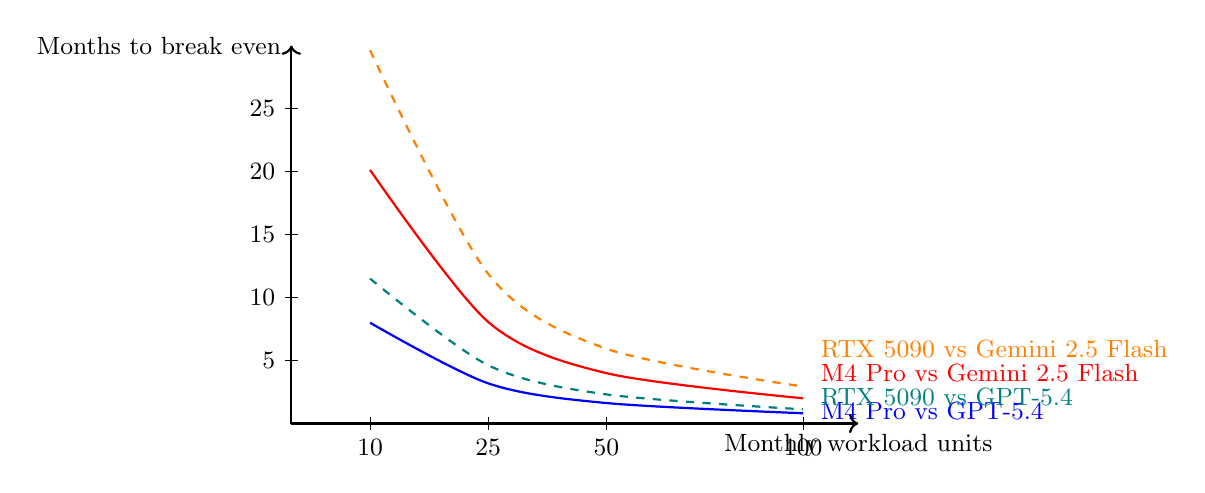
\begin{tikzpicture}[
    font=\small,
    arr/.style={-Latex, thick}
]
\draw[->, thick] (0,0) -- (7.2,0) node[below] {Monthly workload units};
\draw[->, thick] (0,0) -- (0,4.8) node[left] {Months to break even};

\foreach \x/\lab in {1/10,2.5/25,4/50,6.5/100}
  \draw (\x,0.08) -- (\x,-0.08) node[below] {\lab};
\foreach \y/\lab in {0.8/5,1.6/10,2.4/15,3.2/20,4.0/25}
  \draw (0.08,\y) -- (-0.08,\y) node[left] {\lab};

\draw[blue, thick] plot[smooth] coordinates {(1,1.28) (2.5,0.51) (4,0.26) (6.5,0.13)};
\draw[teal, thick, dashed] plot[smooth] coordinates {(1,1.84) (2.5,0.74) (4,0.37) (6.5,0.18)};
\draw[red, thick] plot[smooth] coordinates {(1,3.22) (2.5,1.29) (4,0.64) (6.5,0.32)};
\draw[orange, thick, dashed] plot[smooth] coordinates {(1,4.74) (2.5,1.90) (4,0.95) (6.5,0.47)};

\node[blue, anchor=west] at (6.6,0.16) {M4 Pro vs GPT-5.4};
\node[teal, anchor=west] at (6.6,0.34) {RTX 5090 vs GPT-5.4};
\node[red, anchor=west] at (6.6,0.64) {M4 Pro vs Gemini 2.5 Flash};
\node[orange, anchor=west] at (6.6,0.95) {RTX 5090 vs Gemini 2.5 Flash};
\end{tikzpicture}
\caption{Illustrative break-even curves. Premium APIs are beaten quickly at moderate usage, while very cheap APIs require much heavier sustained volume before local hardware wins on pure cost. Values are computed from the assumptions in Tables~\ref{tab:local_scenarios}, \ref{tab:api_costs}, \ref{tab:breakeven_costs}, and \ref{tab:breakeven_costs_5090}.}
\label{fig:breakeven_curves}
\end{figure}

\subsection{Interpretation}

Three conclusions follow.

First, electricity is not the main driver. Once a local machine exists, the marginal energy cost per million-token-scale workload is extremely small. The dominant economic question is whether the user consumes enough tokens to amortize hardware.

Second, local inference can beat premium hosted APIs surprisingly quickly for heavy users. If a workflow is genuinely in the range of 50 to 100 units per month, which is 100M to 200M total monthly tokens under our definition, even a modest local workstation can recover its cost in a few months relative to premium cloud services.

Third, very cheap hosted APIs are harder to beat. Models such as GPT-5.4 nano or Gemini 2.5 Flash offer such low token prices that local hardware only wins economically when usage is high and sustained. This means the cloud-local decision is not just ``cloud versus local''; it is also ``which cloud tier versus which local capability.''

The second local scenario sharpens this point. A faster GPU setup reduces latency dramatically, but if capital cost rises, break-even against cheap APIs can actually become slower unless the workstation is heavily utilized. In other words, faster local hardware is not automatically cheaper in economic terms; utilization is what matters.

\subsection{A Reusable Calculator}

Readers can reuse the model with their own assumptions. Define:
\begin{itemize}[noitemsep]
    \item $P_{\mathrm{in}}$: API input price per 1M tokens,
    \item $P_{\mathrm{out}}$: API output price per 1M tokens,
    \item $x$: monthly input tokens in millions,
    \item $y$: monthly output tokens in millions,
    \item $H$: hardware cost,
    \item $E$: monthly local electricity plus operating cost.
\end{itemize}

Then monthly cloud spend is:
\begin{equation}
C_{\mathrm{cloud,month}} = xP_{\mathrm{in}} + yP_{\mathrm{out}}
\end{equation}

and monthly local cost is approximately:
\begin{equation}
C_{\mathrm{local,month}} = E + \frac{H}{T}
\end{equation}

if the hardware is amortized over $T$ months. The break-even month count can be estimated as:
\begin{equation}
T_{\mathrm{break-even}} = \frac{H}{(xP_{\mathrm{in}} + yP_{\mathrm{out}}) - E}
\end{equation}

provided the denominator is positive. This formulation makes it easy to substitute a real workload, such as 30M input tokens and 6M output tokens per month, rather than the symmetric 1M-in plus 1M-out unit used for the tables above.

\subsection{Caveats}

This comparison has several important limitations.
\begin{itemize}[noitemsep]
    \item It does not equate model quality. Frontier hosted APIs generally outperform local small open-weight models.
    \item It excludes operational costs such as storage, maintenance, local orchestration software, and the opportunity cost of hardware capital.
    \item It excludes cloud extras such as search, tool execution, and context caching.
    \item It uses one local hardware scenario. Faster or more expensive local hardware changes the break-even line materially.
    \item It treats the workload as symmetric 1M-in plus 1M-out. Real applications often have very different input-output ratios.
\end{itemize}

Even with those caveats, the main systems-level conclusion is robust: once token volume is high enough, local inference becomes economically attractive very quickly, and the non-monetary benefits of privacy, offline operation, and lower latency make the case even stronger.

\section{Conclusion}

The future of agent intelligence depends on escaping the assumption that useful learning must always take the form of expensive online retraining. Prior work in meta-learning, hyper-networks, test-time adaptation, external memory, parameter-efficient tuning, and self-updating language models already points toward a different architecture. The emerging lesson is that competence and plasticity need not live in the same substrate.

Heavy learning can remain offline. Real-time adaptation can happen locally through memory writes, latent modulation, and compact meta-controllers. This is the practical route to adaptive agents on constrained hardware. It aligns with the capabilities of current edge AI stacks, with the privacy demands of personalized systems, and with the need for immediate local response.

When that shift is mature, AI will feel less like a static artifact periodically refreshed from the cloud and more like something that grows in place.

\begin{thebibliography}{99}

\bibitem{finn2017maml}
Chelsea Finn, Pieter Abbeel, and Sergey Levine.
\newblock Model-Agnostic Meta-Learning for Fast Adaptation of Deep Networks.
\newblock In \emph{Proceedings of the 34th International Conference on Machine Learning}, PMLR 70:1126--1135, 2017.
\newblock \url{https://proceedings.mlr.press/v70/finn17a.html}

\bibitem{rajeswaran2019implicit}
Aravind Rajeswaran, Chelsea Finn, Sham Kakade, and Sergey Levine.
\newblock Meta-Learning with Implicit Gradients.
\newblock In \emph{Advances in Neural Information Processing Systems 32}, 2019.
\newblock \url{https://arxiv.org/abs/1909.04630}

\bibitem{ha2016hypernetworks}
David Ha, Andrew Dai, and Quoc V. Le.
\newblock HyperNetworks.
\newblock arXiv:1609.09106, 2016.
\newblock \url{https://arxiv.org/abs/1609.09106}

\bibitem{jia2016dynamic}
Xu Jia, Bert De Brabandere, Tinne Tuytelaars, and Luc Van Gool.
\newblock Dynamic Filter Networks.
\newblock In \emph{Advances in Neural Information Processing Systems 29}, 2016.
\newblock \url{https://proceedings.neurips.cc/paper/2016/hash/8bf1211fd4b7b94528899de0a43b9fb3-Abstract.html}

\bibitem{perez2018film}
Ethan Perez, Florian Strub, Harm de Vries, Vincent Dumoulin, and Aaron Courville.
\newblock FiLM: Visual Reasoning with a General Conditioning Layer.
\newblock In \emph{Proceedings of the AAAI Conference on Artificial Intelligence}, 32(1), 2018.
\newblock \url{https://aaai.org/papers/11671-film-visual-reasoning-with-a-general-conditioning-layer/}

\bibitem{zhmoginov2022hypertransformer}
Andrey Zhmoginov, Mark Sandler, and Maksym Vladymyrov.
\newblock HyperTransformer: Model Generation for Supervised and Semi-Supervised Few-Shot Learning.
\newblock In \emph{Proceedings of the 39th International Conference on Machine Learning}, PMLR 162:27075--27098, 2022.
\newblock \url{https://proceedings.mlr.press/v162/zhmoginov22a.html}

\bibitem{sun2020ttt}
Yu Sun, Xiaolong Wang, Zhuang Liu, John Miller, Alexei Efros, and Moritz Hardt.
\newblock Test-Time Training with Self-Supervision for Generalization under Distribution Shifts.
\newblock In \emph{Proceedings of the 37th International Conference on Machine Learning}, PMLR 119:9229--9248, 2020.
\newblock \url{https://proceedings.mlr.press/v119/sun20b.html}

\bibitem{wang2021tent}
Dequan Wang, Evan Shelhamer, Shaoteng Liu, Bruno Olshausen, and Trevor Darrell.
\newblock Tent: Fully Test-Time Adaptation by Entropy Minimization.
\newblock In \emph{ICLR 2021}.
\newblock \url{https://openreview.net/forum?id=uXl3bZLkr3c}

\bibitem{bartler2022mt3}
Alexander Bartler, Andre B{\"u}hler, Felix Wiewel, Mario D{\"o}bler, and Bin Yang.
\newblock MT3: Meta Test-Time Training for Self-Supervised Test-Time Adaption.
\newblock In \emph{Proceedings of the 25th International Conference on Artificial Intelligence and Statistics}, PMLR 151:3080--3090, 2022.
\newblock \url{https://proceedings.mlr.press/v151/bartler22a.html}

\bibitem{houlsby2019adapters}
Neil Houlsby, Andrei Giurgiu, Stanislaw Jastrzebski, Bruna Morrone, Quentin De Laroussilhe, Andrea Gesmundo, Mona Attariyan, and Sylvain Gelly.
\newblock Parameter-Efficient Transfer Learning for NLP.
\newblock In \emph{Proceedings of the 36th International Conference on Machine Learning}, PMLR 97:2790--2799, 2019.
\newblock \url{https://proceedings.mlr.press/v97/houlsby19a.html}

\bibitem{hu2021lora}
Edward J. Hu, Yelong Shen, Phillip Wallis, Zeyuan Allen-Zhu, Yuanzhi Li, Shean Wang, Lu Wang, and Weizhu Chen.
\newblock LoRA: Low-Rank Adaptation of Large Language Models.
\newblock arXiv:2106.09685, 2021.
\newblock \url{https://arxiv.org/abs/2106.09685}

\bibitem{bansal2022metaadapters}
Trapit Bansal, Salaheddin Alzubi, Tong Wang, Jay-Yoon Lee, and Andrew McCallum.
\newblock Meta-Adapters: Parameter Efficient Few-shot Fine-tuning through Meta-Learning.
\newblock In \emph{Proceedings of the First International Conference on Automated Machine Learning}, PMLR 188:19/1--19/18, 2022.
\newblock \url{https://proceedings.mlr.press/v188/bansal22a.html}

\bibitem{graves2014ntm}
Alex Graves, Greg Wayne, and Ivo Danihelka.
\newblock Neural Turing Machines.
\newblock arXiv:1410.5401, 2014.
\newblock \url{https://arxiv.org/abs/1410.5401}

\bibitem{graves2016dnc}
Alex Graves, Greg Wayne, Malcolm Reynolds, Tim Harley, Ivo Danihelka, Agnieszka Grabska-Barwinska, Sergio G{\'o}mez Colmenarejo, Edward Grefenstette, Tiago Ramalho, John Agapiou, Adri{\`a} Puigdom{\`e}nech Badia, Karl Moritz Hermann, Yori Zwols, Georg Ostrovski, Adam Cain, Helen King, Christopher Summerfield, Phil Blunsom, Koray Kavukcuoglu, and Demis Hassabis.
\newblock Hybrid computing using a neural network with dynamic external memory.
\newblock \emph{Nature}, 538:471--476, 2016.
\newblock \url{https://www.nature.com/articles/nature20101}

\bibitem{santoro2016mann}
Adam Santoro, Sergey Bartunov, Matthew Botvinick, Daan Wierstra, and Timothy Lillicrap.
\newblock One-shot Learning with Memory-Augmented Neural Networks.
\newblock arXiv:1605.06065, 2016.
\newblock \url{https://arxiv.org/abs/1605.06065}

\bibitem{ba2016fastweights}
Jimmy Ba, Geoffrey Hinton, Volodymyr Mnih, Joel Z. Leibo, and Catalin Ionescu.
\newblock Using Fast Weights to Attend to the Recent Past.
\newblock In \emph{Advances in Neural Information Processing Systems 29}, 2016.
\newblock \url{https://papers.nips.cc/paper/2016/file/9f44e956e3a2b7b5598c625fcc802c36-Paper.pdf}

\bibitem{munkhdalai2019mnm}
Tsendsuren Munkhdalai, Alessandro Sordoni, Tong Wang, and Adam Trischler.
\newblock Metalearned Neural Memory.
\newblock In \emph{Advances in Neural Information Processing Systems 32}, 2019.
\newblock \url{https://proceedings.neurips.cc/paper/2019/hash/182bd81ea25270b7d1c2fe8353d17fe6-Abstract.html}

\bibitem{dai2019transformerxl}
Zihang Dai, Zhilin Yang, Yiming Yang, Jaime Carbonell, Quoc V. Le, and Ruslan Salakhutdinov.
\newblock Transformer-XL: Attentive Language Models Beyond a Fixed-Length Context.
\newblock arXiv:1901.02860, 2019.
\newblock \url{https://arxiv.org/abs/1901.02860}

\bibitem{rae2019compressive}
Jack W. Rae, Anna Potapenko, Siddhant M. Jayakumar, and Timothy Lillicrap.
\newblock Compressive Transformers for Long-Range Sequence Modelling.
\newblock arXiv:1911.05507, 2019.
\newblock \url{https://arxiv.org/abs/1911.05507}

\bibitem{wang2024memoryllm}
Yu Wang, Yifan Gao, Xiusi Chen, Haoming Jiang, Shiyang Li, Jingfeng Yang, Qingyu Yin, Zheng Li, Xian Li, Bing Yin, Jingbo Shang, and Julian McAuley.
\newblock MEMORYLLM: Towards Self-Updatable Large Language Models.
\newblock In \emph{Proceedings of the 41st International Conference on Machine Learning}, PMLR 235:50453--50466, 2024.
\newblock \url{https://proceedings.mlr.press/v235/wang24s.html}

\bibitem{tack2024mac}
Jihoon Tack, Soyeong Jeong, Jinheon Baek, and Sung Ju Hwang.
\newblock Online Adaptation of Language Models with a Memory of Amortized Contexts.
\newblock In \emph{Advances in Neural Information Processing Systems 37}, 2024.
\newblock \url{https://papers.nips.cc/paper_files/paper/2024/hash/eaf956b52bae51fbf387b8be4cc3ce18-Abstract-Conference.html}

\bibitem{li2023icl}
Yingcong Li, Muhammed Emrullah Ildiz, Dimitris Papailiopoulos, and Samet Oymak.
\newblock Transformers as Algorithms: Generalization and Stability in In-context Learning.
\newblock In \emph{Proceedings of the 40th International Conference on Machine Learning}, PMLR 202:19565--19594, 2023.
\newblock \url{https://proceedings.mlr.press/v202/li23l.html}

\bibitem{apple_coreml}
Apple.
\newblock Core ML Overview.
\newblock Apple Developer Documentation, accessed April 18, 2026.
\newblock \url{https://developer.apple.com/machine-learning/core-ml/}

\bibitem{apple_wwdc19}
Apple.
\newblock What's New in Machine Learning.
\newblock WWDC19 Session 209, accessed April 18, 2026.
\newblock \url{https://developer.apple.com/videos/play/wwdc2019/209/}

\bibitem{google_edge}
Google.
\newblock Google AI Edge.
\newblock Google AI for Developers, accessed April 18, 2026.
\newblock \url{https://ai.google.dev/edge}

\bibitem{qualcomm_2025}
Qualcomm.
\newblock Snapdragon 8 Elite Gen 5 Product Brief.
\newblock Qualcomm product brief, 2025, accessed April 18, 2026.
\newblock \url{https://www.qualcomm.com/content/dam/qcomm-martech/dm-assets/images/company/news-media/media-center/press-kits/snapdragon-summit-2025-press-kit/day-2-/documents/Snapdragon8EliteGen5_ProductBrief.pdf}

\bibitem{openai_pricing_2026}
OpenAI.
\newblock API Pricing.
\newblock OpenAI documentation, accessed April 19, 2026.
\newblock \url{https://openai.com/api/pricing/}

\bibitem{anthropic_pricing_2026}
Anthropic.
\newblock Claude API Pricing.
\newblock Anthropic documentation, accessed April 19, 2026.
\newblock \url{https://platform.claude.com/docs/en/docs/about-claude/pricing}

\bibitem{google_pricing_2026}
Google.
\newblock Gemini API Pricing.
\newblock Google AI for Developers documentation, accessed April 19, 2026.
\newblock \url{https://ai.google.dev/gemini-api/docs/pricing}

\bibitem{apple_macmini_2024}
Apple.
\newblock Apple's new Mac mini is more mighty, more mini, and built for Apple Intelligence.
\newblock Apple Newsroom, 2024, accessed April 19, 2026.
\newblock \url{https://www.apple.com/newsroom/2024/10/apples-new-mac-mini-is-more-mighty-more-mini-and-built-for-apple-intelligence/}

\bibitem{llamacpp_m4pro_bench}
ggml-org community.
\newblock llama.cpp benchmark discussion for Apple M4 Pro.
\newblock GitHub Discussions, accessed April 19, 2026.
\newblock \url{https://github.com/ggml-org/llama.cpp/discussions/12985}

\bibitem{eia_2025}
U.S. Energy Information Administration.
\newblock Short-Term Energy Outlook, Table SF02.
\newblock EIA report, accessed April 19, 2026.
\newblock \url{https://www.eia.gov/outlooks/steo/pdf/sf02.pdf}

\bibitem{nvidia_5090_specs}
NVIDIA.
\newblock GeForce RTX 5090.
\newblock NVIDIA product page, accessed April 19, 2026.
\newblock \url{https://www.nvidia.com/en-us/geforce/graphics-cards/50-series/rtx-5090/}

\bibitem{nvidia_5090_price}
NVIDIA.
\newblock GeForce RTX 5090 Founders Edition.
\newblock NVIDIA Marketplace product page, accessed April 19, 2026.
\newblock \url{https://marketplace.nvidia.com/en-us/consumer/graphics-cards/geforce-rtx-5090-founders-edition/}

\bibitem{llamacpp_5090_bench}
ggml-org community.
\newblock llama.cpp benchmark discussion for RTX 5090.
\newblock GitHub Discussions, accessed April 19, 2026.
\newblock \url{https://github.com/ggml-org/llama.cpp/discussions/15013}

\end{thebibliography}

\end{document}
